\documentclass[11pt]{article}
\usepackage[a4paper,landscape,margin=1.0cm]{geometry}
\usepackage{amsmath,amssymb}
\usepackage{tikz}
\usetikzlibrary{positioning,arrows.meta,calc,fit,backgrounds}
\pagestyle{empty}
\setlength{\parindent}{0pt}
\definecolor{cP}{HTML}{1F5FAD}
\definecolor{cV}{HTML}{B4462A}
\definecolor{cG}{HTML}{2E7D4F}
\definecolor{cQ}{HTML}{7A3DA8}
\definecolor{bg}{HTML}{F4F6FA}
\newcommand{\F}{\mathbb F}
\newcommand{\K}{\mathbb K}
\tikzset{
 pbox/.style={draw=cP!60,fill=cP!6,rounded corners=3pt,inner sep=4pt,align=left,font=\footnotesize,text width=8.1cm,anchor=west},
 vbox/.style={draw=cV!60,fill=cV!6,rounded corners=3pt,inner sep=4pt,align=left,font=\footnotesize,text width=7.6cm,anchor=west},
 stepn/.style={circle,fill=black!75,text=white,font=\scriptsize\bfseries,inner sep=1.5pt,minimum size=0.5cm},
 msgP/.style={-{Stealth[length=2.6mm]},very thick,cP},
 msgV/.style={-{Stealth[length=2.6mm]},very thick,cV},
 mlab/.style={font=\footnotesize,fill=white,inner sep=2pt,align=center},
 cell/.style={draw=black!60,minimum width=0.9cm,minimum height=0.55cm,font=\footnotesize,fill=white,inner sep=1pt},
 qcell/.style={cell,fill=cQ!20,draw=cQ,thick},
 gnode/.style={rounded corners=2pt,draw=cG,thick,fill=cG!10,font=\scriptsize,inner sep=2pt,align=center},
 arr/.style={-{Stealth[length=2mm]},thick},
 box/.style={draw=black!40,rounded corners=3pt,fill=white,inner sep=5pt,align=left},
 phase/.style={font=\scriptsize\bfseries,text=black!55,rotate=90,anchor=south},
}
\begin{document}
%=====================================================================
% PAGE 1 : the message flow and the state of both parties
%=====================================================================
\begin{center}
{\LARGE\bfseries SPARK, step by step: how the state evolves with each message}\\[2pt]
{\normalsize left: what the prover holds \quad$\cdot$\quad middle: the message \quad$\cdot$\quad right: what the verifier knows after it}
\end{center}
\vspace{-4pt}
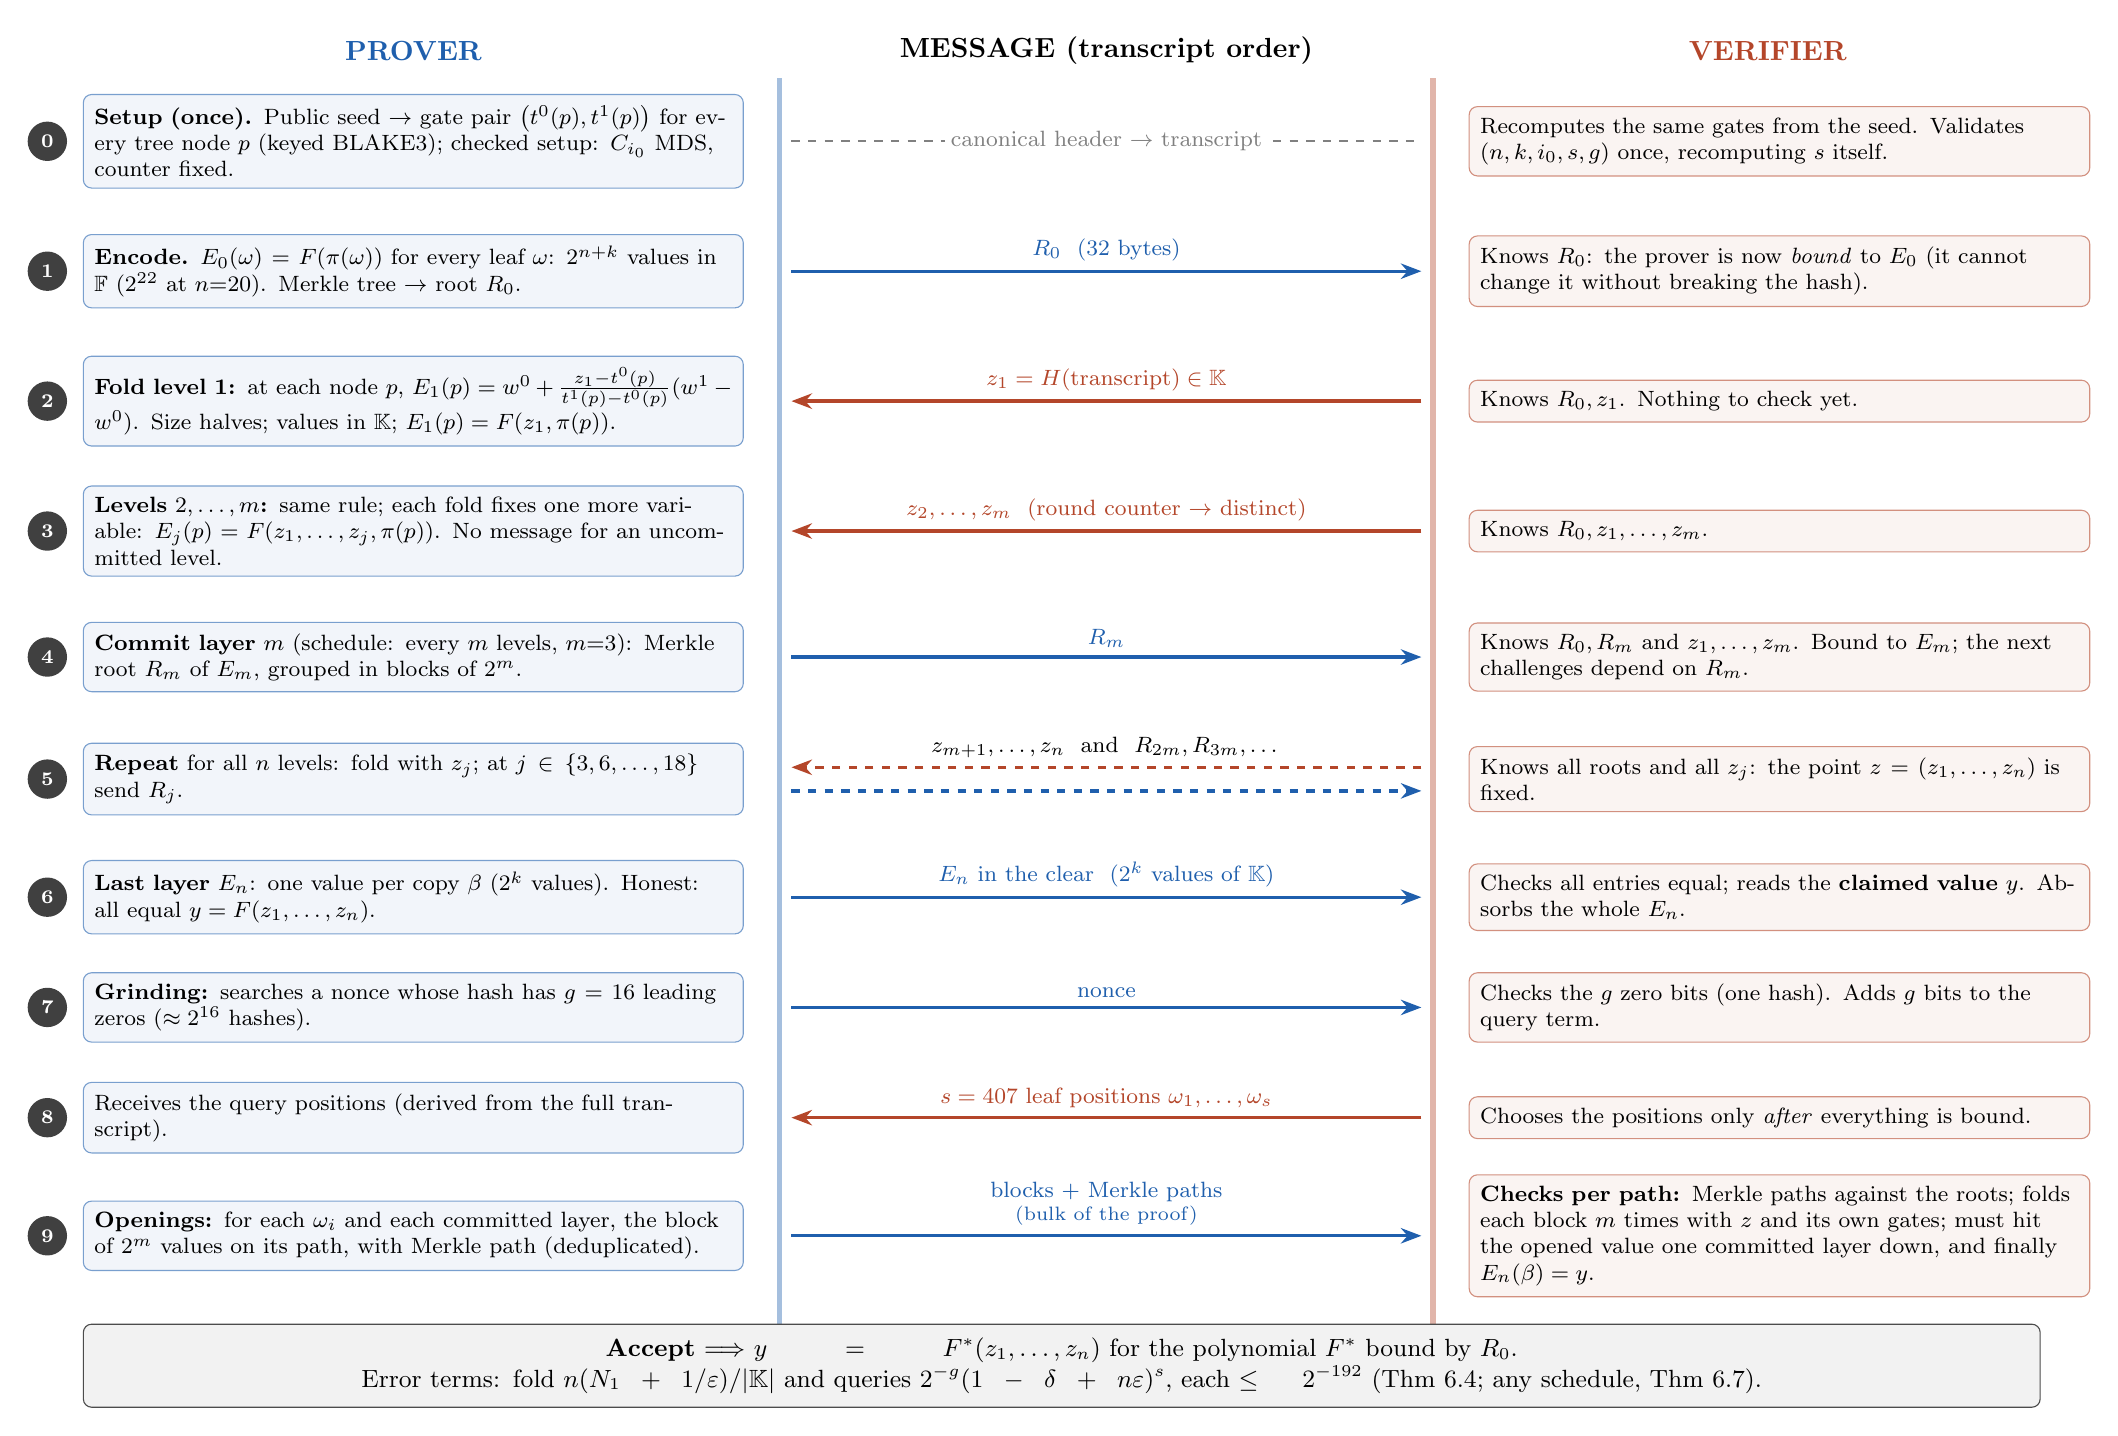
\begin{tikzpicture}[x=1cm,y=1cm]
\def\xP{0}\def\xM{9.0}\def\xMe{17.0}\def\xV{17.6}
\node[font=\bfseries,text=cP] at (4.2,0.55) {PROVER};
\node[font=\bfseries] at (13.0,0.55) {MESSAGE (transcript order)};
\node[font=\bfseries,text=cV] at (21.4,0.55) {VERIFIER};
\draw[cP!40,line width=2pt] (8.85,0.2)--(8.85,-16.6);
\draw[cV!40,line width=2pt] (17.15,0.2)--(17.15,-16.6);

% ---- row 0 : setup
\node[pbox] at (\xP,-0.6) {\textbf{Setup (once).} Public seed $\to$ gate pair $\bigl(t^0(p),t^1(p)\bigr)$ for every tree node $p$ (keyed BLAKE3); checked setup: $C_{i_0}$ MDS, counter fixed.};
\node[vbox] at (\xV,-0.6) {Recomputes the same gates from the seed. Validates $(n,k,i_0,s,g)$ once, recomputing $s$ itself.};
\draw[black!50,dashed,thick] (\xM,-0.6)--(\xMe,-0.6) node[mlab,midway] {canonical header $\to$ transcript};
\node[stepn] at (-0.45,-0.6) {0};

% ---- row 1 : commit
\node[pbox] at (\xP,-2.25) {\textbf{Encode.} $E_0(\omega)=F(\pi(\omega))$ for every leaf $\omega$: $2^{n+k}$ values in $\F$ ($2^{22}$ at $n{=}20$). Merkle tree $\to$ root $R_0$.};
\draw[msgP] (\xM,-2.25)--(\xMe,-2.25) node[mlab,midway,above=1pt] {$R_0$\ \ (32 bytes)};
\node[vbox] at (\xV,-2.25) {Knows $R_0$: the prover is now \emph{bound} to $E_0$ (it cannot change it without breaking the hash).};
\node[stepn] at (-0.45,-2.25) {1};

% ---- row 2 : first challenge
\node[pbox] at (\xP,-3.9) {\textbf{Fold level 1:} at each node $p$,\ $E_1(p)=w^0+\tfrac{z_1-t^0(p)}{t^1(p)-t^0(p)}(w^1-w^0)$. Size halves; values in $\K$; $E_1(p)=F(z_1,\pi(p))$.};
\draw[msgV] (\xMe,-3.9)--(\xM,-3.9) node[mlab,midway,above=1pt] {$z_1=H(\text{transcript})\in\K$};
\node[vbox] at (\xV,-3.9) {Knows $R_0,z_1$. Nothing to check yet.};
\node[stepn] at (-0.45,-3.9) {2};

% ---- row 3 : more folds
\node[pbox] at (\xP,-5.55) {\textbf{Levels $2,\dots,m$:} same rule; each fold fixes one more variable: $E_j(p)=F(z_1,\dots,z_j,\pi(p))$. No message for an uncommitted level.};
\draw[msgV] (\xMe,-5.55)--(\xM,-5.55) node[mlab,midway,above=1pt] {$z_2,\dots,z_m$\ \ (round counter $\to$ distinct)};
\node[vbox] at (\xV,-5.55) {Knows $R_0,z_1,\dots,z_m$.};
\node[stepn] at (-0.45,-5.55) {3};

% ---- row 4 : committed layer
\node[pbox] at (\xP,-7.15) {\textbf{Commit layer $m$} (schedule: every $m$ levels, $m{=}3$): Merkle root $R_m$ of $E_m$, grouped in blocks of $2^m$.};
\draw[msgP] (\xM,-7.15)--(\xMe,-7.15) node[mlab,midway,above=1pt] {$R_m$};
\node[vbox] at (\xV,-7.15) {Knows $R_0,R_m$ and $z_1,\dots,z_m$. Bound to $E_m$; the next challenges depend on $R_m$.};
\node[stepn] at (-0.45,-7.15) {4};

% ---- row 5 : loop
\node[pbox] at (\xP,-8.7) {\textbf{Repeat} for all $n$ levels: fold with $z_j$; at $j\in\{3,6,\dots,18\}$ send $R_j$.};
\draw[msgV,dashed] (\xMe,-8.55)--(\xM,-8.55);\draw[msgP,dashed] (\xM,-8.85)--(\xMe,-8.85);
\node[mlab] at (13,-8.3) {$z_{m+1},\dots,z_n$\ \ and\ \ $R_{2m},R_{3m},\dots$};
\node[vbox] at (\xV,-8.7) {Knows all roots and all $z_j$: the point $z=(z_1,\dots,z_n)$ is fixed.};
\node[stepn] at (-0.45,-8.7) {5};

% ---- row 6 : last layer
\node[pbox] at (\xP,-10.2) {\textbf{Last layer} $E_n$: one value per copy $\beta$ ($2^k$ values). Honest: all equal $y=F(z_1,\dots,z_n)$.};
\draw[msgP] (\xM,-10.2)--(\xMe,-10.2) node[mlab,midway,above=1pt] {$E_n$ in the clear\ \ ($2^k$ values of $\K$)};
\node[vbox] at (\xV,-10.2) {Checks all entries equal; reads the \textbf{claimed value} $y$. Absorbs the whole $E_n$.};
\node[stepn] at (-0.45,-10.2) {6};

% ---- row 7 : grinding
\node[pbox] at (\xP,-11.6) {\textbf{Grinding:} searches a nonce whose hash has $g=16$ leading zeros ($\approx2^{16}$ hashes).};
\draw[msgP] (\xM,-11.6)--(\xMe,-11.6) node[mlab,midway,above=1pt] {nonce};
\node[vbox] at (\xV,-11.6) {Checks the $g$ zero bits (one hash). Adds $g$ bits to the query term.};
\node[stepn] at (-0.45,-11.6) {7};

% ---- row 8 : queries
\node[pbox] at (\xP,-13.0) {Receives the query positions (derived from the full transcript).};
\draw[msgV] (\xMe,-13.0)--(\xM,-13.0) node[mlab,midway,above=1pt] {$s=407$ leaf positions $\omega_1,\dots,\omega_s$};
\node[vbox] at (\xV,-13.0) {Chooses the positions only \emph{after} everything is bound.};
\node[stepn] at (-0.45,-13.0) {8};

% ---- row 9 : openings
\node[pbox] at (\xP,-14.5) {\textbf{Openings:} for each $\omega_i$ and each committed layer, the block of $2^m$ values on its path, with Merkle path (deduplicated).};
\draw[msgP] (\xM,-14.5)--(\xMe,-14.5) node[mlab,midway,above=1pt] {blocks + Merkle paths\\[-1pt]{\scriptsize (bulk of the proof)}};
\node[vbox] at (\xV,-14.5) {\textbf{Checks per path:} Merkle paths against the roots; folds each block $m$ times with $z$ and its own gates; must hit the opened value one committed layer down, and finally $E_n(\beta)=y$.};
\node[stepn] at (-0.45,-14.5) {9};

% ---- row 10 : decision
\node[draw=black!70,fill=black!5,rounded corners=3pt,inner sep=5pt,font=\small,align=center,text width=24.5cm,anchor=west] at (0,-16.15)
 {\textbf{Accept} $\Longrightarrow$ $y=F^{*}(z_1,\dots,z_n)$ for the polynomial $F^{*}$ bound by $R_0$.\\ Error terms: fold $n(N_1+1/\varepsilon)/|\K|$ and queries $2^{-g}(1-\delta+n\varepsilon)^{s}$, each $\le2^{-192}$ (Thm 6.4; any schedule, Thm 6.7).};
\end{tikzpicture}

\newpage
%=====================================================================
% PAGE 2 : the running example, numbers at every step
%=====================================================================
\begin{center}
{\LARGE\bfseries Worked example over $\F_7$: the tables after each message}\\[2pt]
{\normalsize $F(x_1,x_2)=3+2x_1+5x_2+x_1x_2$, \ $n=2$, \ $k=1$ (two copies $\beta=0,1$), \ challenges $z_1=3,\ z_2=2$}
\end{center}
\vspace{-6pt}
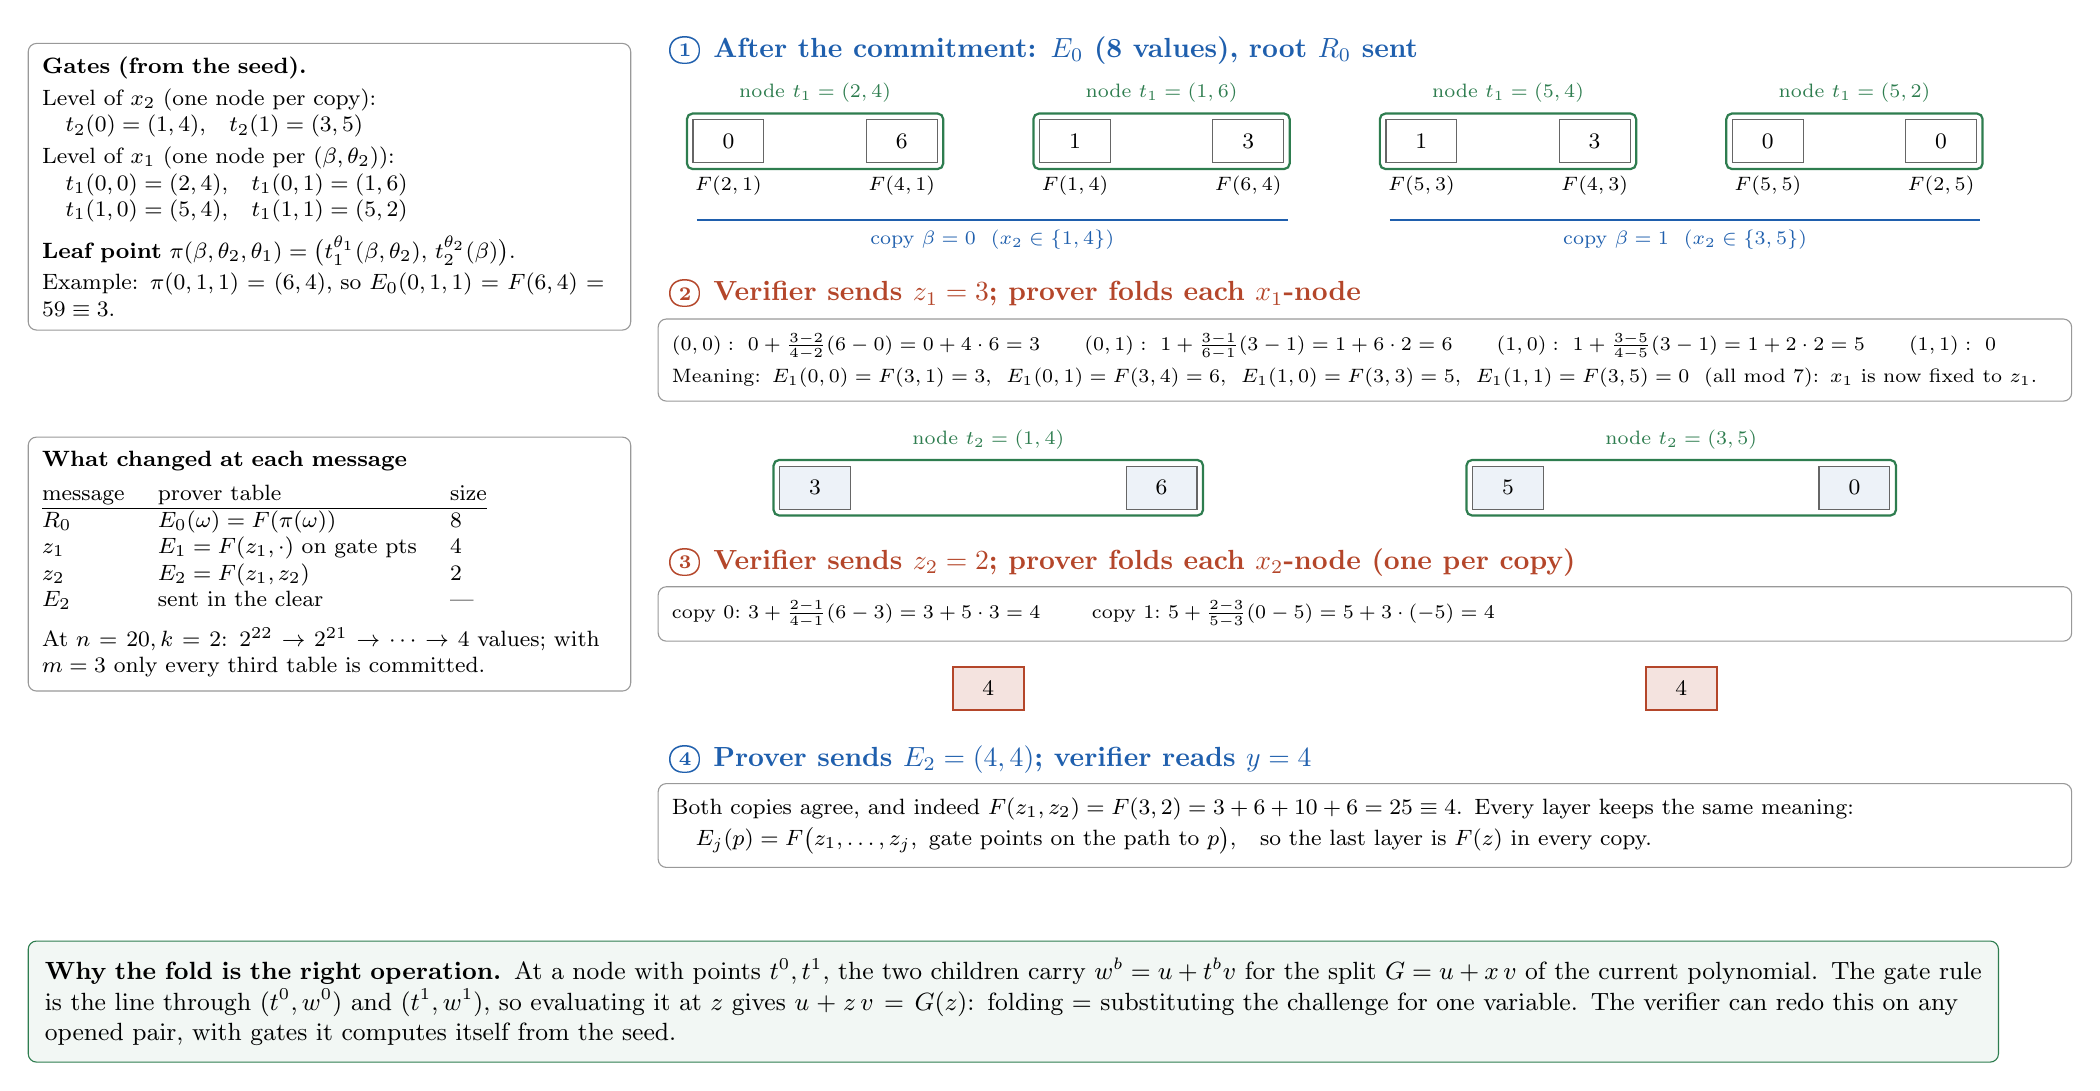
\begin{tikzpicture}[x=1cm,y=1cm]
% ------------- tree of gates (left)
\node[box,font=\footnotesize,text width=7.3cm,anchor=north west] at (0,0) {
\textbf{Gates (from the seed).}\\[2pt]
Level of $x_2$ (one node per copy):\\
\quad $t_2(0)=(1,4)$,\quad $t_2(1)=(3,5)$\\[2pt]
Level of $x_1$ (one node per $(\beta,\theta_2)$):\\
\quad $t_1(0,0)=(2,4)$,\quad $t_1(0,1)=(1,6)$\\
\quad $t_1(1,0)=(5,4)$,\quad $t_1(1,1)=(5,2)$\\[4pt]
\textbf{Leaf point} $\pi(\beta,\theta_2,\theta_1)=\bigl(t_1^{\theta_1}(\beta,\theta_2),\,t_2^{\theta_2}(\beta)\bigr)$.\\[2pt]
Example: $\pi(0,1,1)=(6,4)$, so $E_0(0,1,1)=F(6,4)=59\equiv3$.};

% ------------- STEP 1 : E0
\def\X{8.4}\def\W{2.2}
\node[font=\bfseries,text=cP,anchor=west] at (8.0,-0.1) {\textcircled{\scriptsize 1}\ After the commitment: $E_0$ (8 values), root $R_0$ sent};
\foreach \v/\i/\lab in {0/0/{F(2,1)},6/1/{F(4,1)},1/2/{F(1,4)},3/3/{F(6,4)},1/4/{F(5,3)},3/5/{F(4,3)},0/6/{F(5,5)},0/7/{F(2,5)}}{
  \node[cell] (a\i) at (\X+0.5+\i*\W,-1.25) {$\v$};
  \node[font=\scriptsize,below=1pt of a\i] {$\lab$};}
\foreach \i/\j/\t in {0/1/{(2,4)},2/3/{(1,6)},4/5/{(5,4)},6/7/{(5,2)}}{
 \node[draw=cG,thick,rounded corners=2pt,fit=(a\i)(a\j),inner sep=2pt] (g\i) {};
 \node[font=\scriptsize,text=cG,above=0pt of g\i] {node $t_1=\t$};}
\draw[thick,cP] (\X+0.1,-2.25)--(\X+7.6,-2.25) node[midway,below,font=\scriptsize] {copy $\beta=0$\ \ ($x_2\in\{1,4\}$)};
\draw[thick,cP] (\X+8.9,-2.25)--(\X+16.4,-2.25) node[midway,below,font=\scriptsize] {copy $\beta=1$\ \ ($x_2\in\{3,5\}$)};

% ------------- STEP 2 : fold z1
\node[font=\bfseries,text=cV,anchor=west] at (8.0,-3.2) {\textcircled{\scriptsize 2}\ Verifier sends $z_1=3$;\ prover folds each $x_1$-node};
\node[box,font=\scriptsize,anchor=north west,text width=17.6cm] at (8.0,-3.5) {
$(0,0):\ 0+\tfrac{3-2}{4-2}(6-0)=0+4\cdot6=3$\qquad
$(0,1):\ 1+\tfrac{3-1}{6-1}(3-1)=1+6\cdot2=6$\qquad
$(1,0):\ 1+\tfrac{3-5}{4-5}(3-1)=1+2\cdot2=5$\qquad
$(1,1):\ 0$\\[2pt]
Meaning: $E_1(0,0)=F(3,1)=3$,\ \ $E_1(0,1)=F(3,4)=6$,\ \ $E_1(1,0)=F(3,3)=5$,\ \ $E_1(1,1)=F(3,5)=0$\ \ (all mod 7): $x_1$ is now fixed to $z_1$.};
\foreach \v/\i in {3/0,6/1,5/2,0/3}{ \node[cell,fill=cP!8] (b\i) at (\X+0.5+\W/2+\i*2*\W,-5.65) {$\v$}; }

\foreach \i/\j/\t in {0/1/{(1,4)},2/3/{(3,5)}}{
 \node[draw=cG,thick,rounded corners=2pt,fit=(b\i)(b\j),inner sep=2pt] (h\i) {};
 \node[font=\scriptsize,text=cG,above=0pt of h\i] {node $t_2=\t$};}

% ------------- STEP 3 : fold z2
\node[font=\bfseries,text=cV,anchor=west] at (8.0,-6.6) {\textcircled{\scriptsize 3}\ Verifier sends $z_2=2$;\ prover folds each $x_2$-node (one per copy)};
\node[box,font=\scriptsize,anchor=north west,text width=17.6cm] at (8.0,-6.9) {
copy 0:\ $3+\tfrac{2-1}{4-1}(6-3)=3+5\cdot3=4$ \qquad copy 1:\ $5+\tfrac{2-3}{5-3}(0-5)=5+3\cdot(-5)=4$};
\foreach \v/\i in {4/0,4/1}{ \node[cell,fill=cV!15,draw=cV,thick] (c\i) at (\X+0.5+1.5*\W+\i*4*\W,-8.2) {$\v$}; }


% ------------- STEP 4 : last layer
\node[font=\bfseries,text=cP,anchor=west] at (8.0,-9.1) {\textcircled{\scriptsize 4}\ Prover sends $E_2=(4,4)$;\ verifier reads $y=4$};
\node[box,font=\footnotesize,anchor=north west,text width=17.6cm] at (8.0,-9.4) {
Both copies agree, and indeed $F(z_1,z_2)=F(3,2)=3+6+10+6=25\equiv4$. Every layer keeps the same meaning:\\[2pt]
\hspace*{1em}$E_j(p)=F\bigl(z_1,\dots,z_j,\ \text{gate points on the path to }p\bigr)$,\quad so the last layer is $F(z)$ in every copy.};

% ------------- left column: evolution summary
\node[box,font=\footnotesize,text width=7.3cm,anchor=north west] at (0,-5.0) {
\textbf{What changed at each message}\\[3pt]
\begin{tabular}{@{}lll@{}}
message & prover table & size\\\hline
$R_0$ & $E_0(\omega)=F(\pi(\omega))$ & 8\\
$z_1$ & $E_1=F(z_1,\cdot)$ on gate pts & 4\\
$z_2$ & $E_2=F(z_1,z_2)$ & 2\\
$E_2$ & sent in the clear & ---\\
\end{tabular}\\[4pt]
At $n=20,k=2$: $2^{22}\to2^{21}\to\cdots\to4$ values; with $m=3$ only every third table is committed.};

% ------------- bottom: closed form box
\node[draw=cG,fill=cG!6,rounded corners=3pt,inner sep=6pt,font=\small,align=left,text width=24.6cm,anchor=north west] at (0,-11.4) {
\textbf{Why the fold is the right operation.} At a node with points $t^0,t^1$, the two children carry $w^b=u+t^b v$ for the split $G=u+x\,v$ of the current polynomial. The gate rule is the line through $(t^0,w^0)$ and $(t^1,w^1)$, so evaluating it at $z$ gives $u+z\,v=G(z)$: folding = substituting the challenge for one variable. The verifier can redo this on any opened pair, with gates it computes itself from the seed.};
\end{tikzpicture}

\newpage
%=====================================================================
% PAGE 3 : one query in the example, and the real-size timeline
%=====================================================================
\begin{center}
{\LARGE\bfseries The query phase, and the real sizes at each round}
\end{center}
\vspace{-6pt}
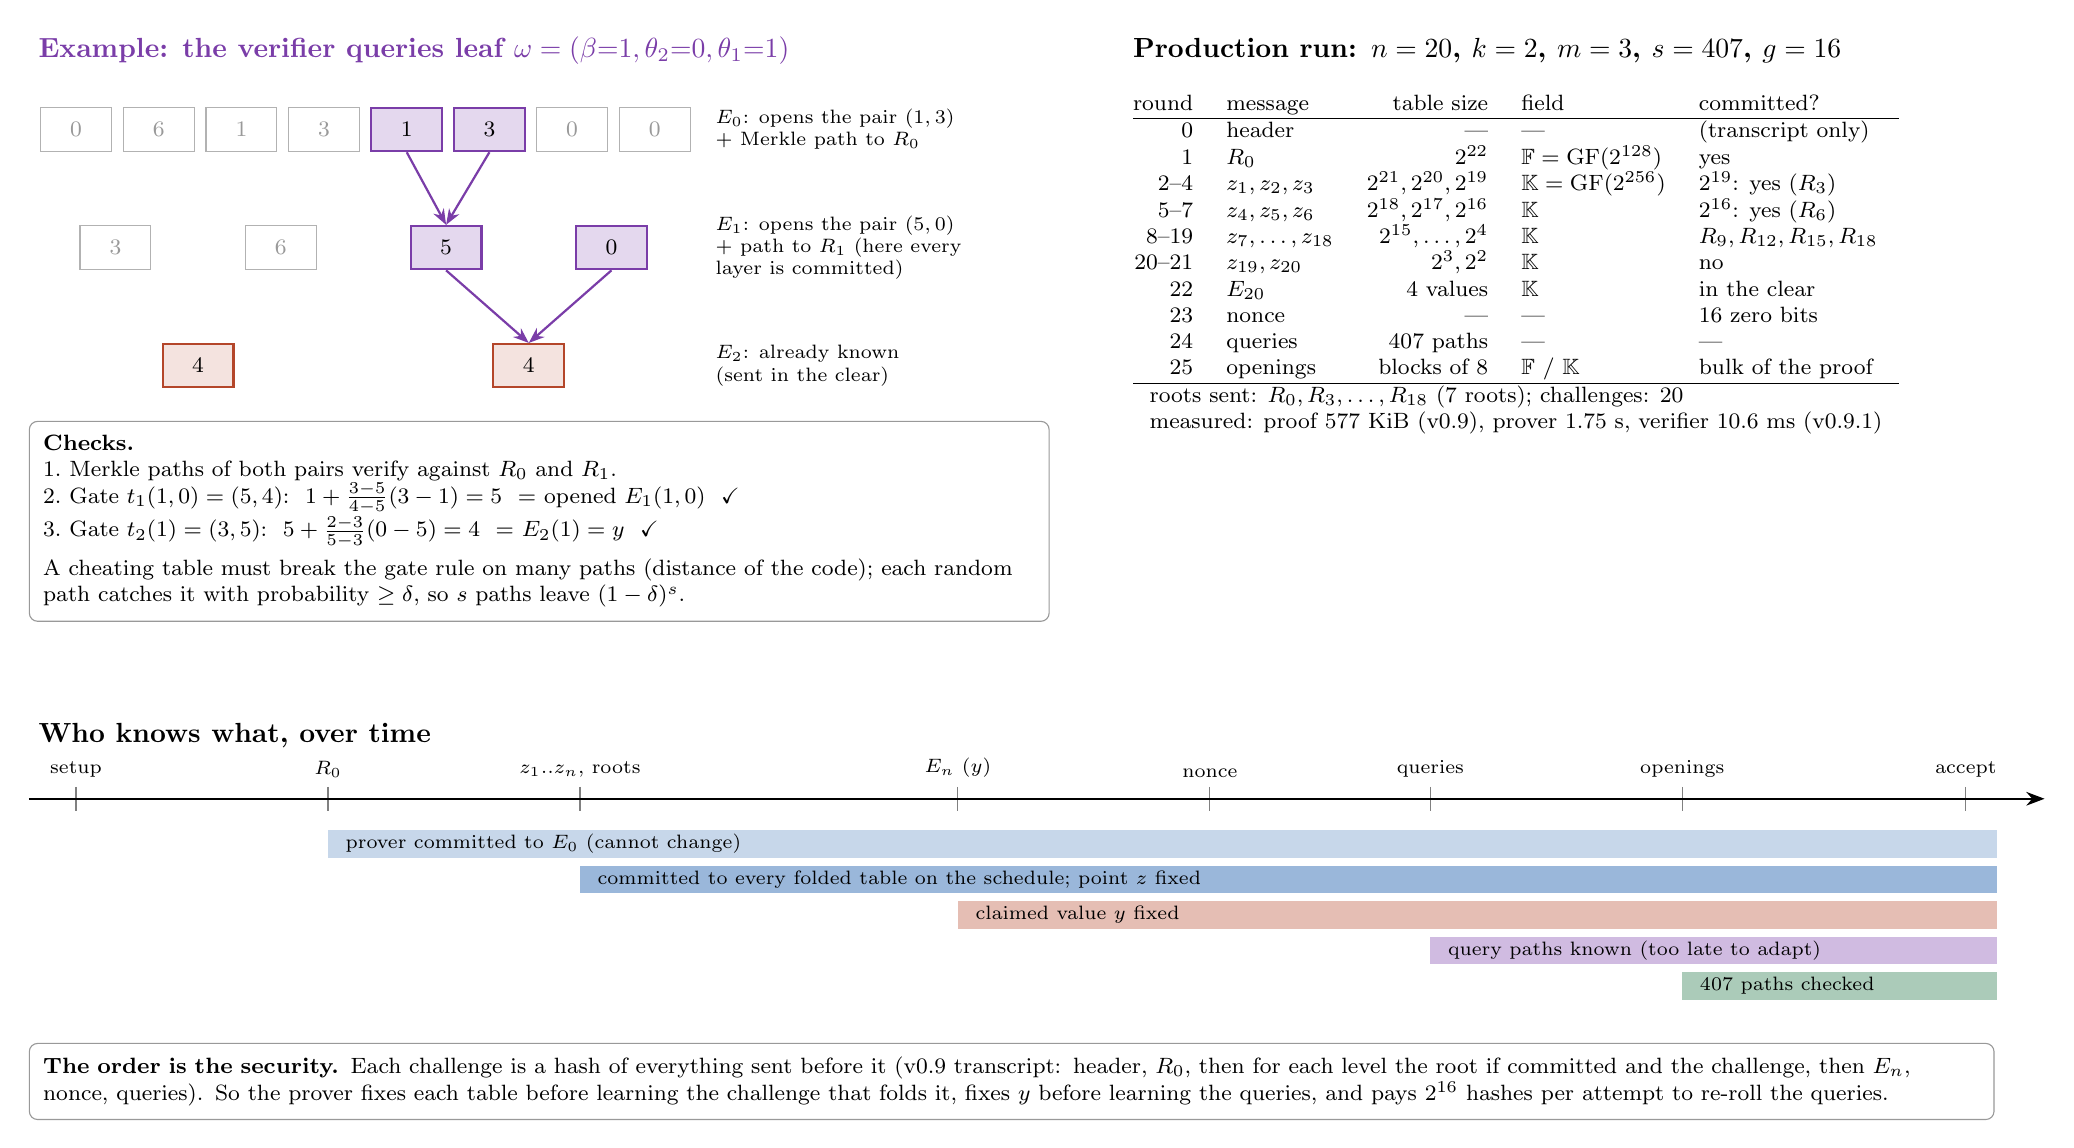
\begin{tikzpicture}[x=1cm,y=1cm]
% ---------------- example query
\node[font=\bfseries,text=cQ,anchor=west] at (0,0) {Example: the verifier queries leaf $\omega=(\beta{=}1,\theta_2{=}0,\theta_1{=}1)$};
\foreach \v/\i in {0/0,6/1,1/2,3/3,1/4,3/5,0/6,0/7}{
 \ifnum\i=4 \node[qcell] (q\i) at (0.6+\i*1.05,-1.0) {$\v$};
 \else\ifnum\i=5 \node[qcell] (q\i) at (0.6+\i*1.05,-1.0) {$\v$};
 \else \node[cell,draw=black!30,text=black!40] (q\i) at (0.6+\i*1.05,-1.0) {$\v$}; \fi\fi}
\node[font=\scriptsize,anchor=west,align=left] at (8.6,-1.0) {$E_0$: opens the pair $(1,3)$\\+ Merkle path to $R_0$};
\foreach \v/\i in {3/0,6/1,5/2,0/3}{
 \ifnum\i=2 \node[qcell] (r\i) at (1.1+\i*2.1,-2.5) {$\v$};
 \else\ifnum\i=3 \node[qcell] (r\i) at (1.1+\i*2.1,-2.5) {$\v$};
 \else \node[cell,draw=black!30,text=black!40] (r\i) at (1.1+\i*2.1,-2.5) {$\v$}; \fi\fi}
\draw[arr,cQ] (q4.south)--(r2.north); \draw[arr,cQ] (q5.south)--(r2.north);
\node[font=\scriptsize,anchor=west,align=left] at (8.6,-2.5) {$E_1$: opens the pair $(5,0)$\\+ path to $R_1$ (here every\\layer is committed)};
\foreach \v/\i in {4/0,4/1}{ \node[cell,fill=cV!15,draw=cV,thick] (s\i) at (2.15+\i*4.2,-4.0) {$\v$}; }
\draw[arr,cQ] (r2.south)--(s1.north); \draw[arr,cQ] (r3.south)--(s1.north);
\node[font=\scriptsize,anchor=west,align=left] at (8.6,-4.0) {$E_2$: already known\\(sent in the clear)};
\node[box,font=\footnotesize,anchor=north west,text width=12.6cm] at (0,-4.7) {
\textbf{Checks.}\\
1.\ Merkle paths of both pairs verify against $R_0$ and $R_1$.\\
2.\ Gate $t_1(1,0)=(5,4)$:\ \ $1+\frac{3-5}{4-5}(3-1)=5$ \ $=$ opened $E_1(1,0)$ \ \checkmark\\
3.\ Gate $t_2(1)=(3,5)$:\ \ $5+\frac{2-3}{5-3}(0-5)=4$ \ $=$ $E_2(1)=y$ \ \checkmark\\[3pt]
A cheating table must break the gate rule on many paths (distance of the code); each random path catches it with probability $\ge\delta$, so $s$ paths leave $(1-\delta)^s$.};

% ---------------- real sizes timeline
\node[font=\bfseries,anchor=west] at (13.9,0) {Production run: $n=20$, $k=2$, $m=3$, $s=407$, $g=16$};
\node[anchor=north west,font=\footnotesize] at (13.9,-0.4) {
\begin{tabular}{@{}rlrll@{}}
round & message & table size & field & committed?\\\hline
0 & header & --- & --- & (transcript only)\\
1 & $R_0$ & $2^{22}$ & $\F=\mathrm{GF}(2^{128})$ & yes\\
2--4 & $z_1,z_2,z_3$ & $2^{21},2^{20},2^{19}$ & $\K=\mathrm{GF}(2^{256})$ & $2^{19}$: yes ($R_3$)\\
5--7 & $z_4,z_5,z_6$ & $2^{18},2^{17},2^{16}$ & $\K$ & $2^{16}$: yes ($R_6$)\\
8--19 & $z_7,\dots,z_{18}$ & $2^{15},\dots,2^{4}$ & $\K$ & $R_9,R_{12},R_{15},R_{18}$\\
20--21 & $z_{19},z_{20}$ & $2^{3},2^{2}$ & $\K$ & no\\
22 & $E_{20}$ & $4$ values & $\K$ & in the clear\\
23 & nonce & --- & --- & $16$ zero bits\\
24 & queries & $407$ paths & --- & ---\\
25 & openings & blocks of 8 & $\F$ / $\K$ & bulk of the proof\\\hline
\multicolumn{5}{l}{roots sent: $R_0,R_3,\dots,R_{18}$ (7 roots); challenges: 20}\\
\multicolumn{5}{l}{measured: proof 577 KiB (v0.9), prover 1.75 s, verifier 10.6 ms (v0.9.1)}\\
\end{tabular}};

% ---------------- state of knowledge bar
\node[font=\bfseries,anchor=west] at (0,-8.7) {Who knows what, over time};
\begin{scope}[shift={(0,-9.5)}]
 \foreach \x/\t in {0/{setup},3.2/{$R_0$},6.4/{$z_1..z_n$, roots},11.2/{$E_n$ ($y$)},14.4/{nonce},17.2/{queries},20.4/{openings},24.0/{accept}}{
   \draw[black!50] (\x+0.6,0.15)--(\x+0.6,-0.15); \node[font=\scriptsize,above] at (\x+0.6,0.15) {\t};}
 \draw[thick,-{Stealth}] (0,0)--(25.6,0);
 \fill[cP!25] (3.8,-0.4) rectangle (25.0,-0.75); \node[font=\scriptsize,anchor=west] at (3.9,-0.575) {prover committed to $E_0$ (cannot change)};
 \fill[cP!45] (7.0,-0.85) rectangle (25.0,-1.2); \node[font=\scriptsize,anchor=west] at (7.1,-1.025) {committed to every folded table on the schedule; point $z$ fixed};
 \fill[cV!35] (11.8,-1.3) rectangle (25.0,-1.65); \node[font=\scriptsize,anchor=west] at (11.9,-1.475) {claimed value $y$ fixed};
 \fill[cQ!35] (17.8,-1.75) rectangle (25.0,-2.1); \node[font=\scriptsize,anchor=west] at (17.9,-1.925) {query paths known (too late to adapt)};
 \fill[cG!40] (21.0,-2.2) rectangle (25.0,-2.55); \node[font=\scriptsize,anchor=west] at (21.1,-2.375) {$407$ paths checked};
\end{scope}
\node[box,font=\footnotesize,anchor=north west,text width=24.6cm] at (0,-12.6) {
\textbf{The order is the security.} Each challenge is a hash of everything sent before it (v0.9 transcript: header, $R_0$, then for each level the root if committed and the challenge, then $E_n$, nonce, queries). So the prover fixes each table before learning the challenge that folds it, fixes $y$ before learning the queries, and pays $2^{16}$ hashes per attempt to re-roll the queries.};
\end{tikzpicture}
\end{document}
